\documentclass[aspectratio=169]{beamer}
\usetheme{Madrid}
\usefonttheme{structurebold}
\usefonttheme[onlymath]{serif}

\definecolor{BKTemplate}{rgb}{0.11765, 0.30588, 0.47451}
\usecolortheme[named=BKTemplate]{structure}
\setbeamercolor{title}{fg=BKTemplate,bg=}
\setbeamertemplate{caption}[numbered]

% Engine-adaptive font configuration
\usepackage{iftex}
\ifLuaTeX
  \usepackage{fontspec}
  \setmainfont{Noto Sans}
  \setsansfont{Noto Sans}
  \setmonofont{Noto Sans Mono}
\else\ifXeTeX
  \usepackage{fontspec}
  \setmainfont{Noto Sans}
  \setsansfont{Noto Sans}
  \setmonofont{Noto Sans Mono}
\else
  \usepackage[utf8]{inputenc}
  \usepackage[T5,T1]{fontenc}
\fi\fi

\usepackage[english,vietnamese]{babel}
\usepackage{url}
\usepackage{booktabs}
\usepackage{array}
\usepackage{amsfonts}
\usepackage{amsmath}
\usepackage{mathtools}
\usepackage{xcolor}
\usepackage{colortbl}
\usepackage{graphicx}
\usepackage{tikz}
\usetikzlibrary{shapes,arrows,positioning,calc,decorations.pathreplacing}
\usepackage{listings}

\newcolumntype{L}[1]{>{\raggedright\arraybackslash}p{#1}}

% Code listing configuration
\lstset{
  basicstyle=\ttfamily\fontsize{6.8}{8.2}\selectfont,
  keywordstyle=\color{blue}\bfseries,
  commentstyle=\color{gray!70!black},
  stringstyle=\color{red!70!black},
  breaklines=true,
  frame=single,
  backgroundcolor=\color{BKTemplate!5},
  rulecolor=\color{BKTemplate!40},
  tabsize=2,
  showstringspaces=false,
  columns=fullflexible,
  keepspaces=true
}
\lstdefinestyle{dense}{basicstyle=\ttfamily\fontsize{6.2}{7.2}\selectfont}

% HCMUT backgrounds (skipped silently if the image files are missing)
\newcommand{\setHCMUTFrontBackground}{%
  \setbeamertemplate{background canvas}{%
    \IfFileExists{images/FrontBackground.pdf}{%
      
\includegraphics[width=\paperwidth,height=\paperheight]{images/FrontBackground.pdf}%
    }{}%
  }%
}
\newcommand{\setHCMUTInnerBackground}{%
  \setbeamertemplate{background canvas}{%
    \IfFileExists{images/Background.pdf}{%
      
\includegraphics[width=\paperwidth,height=\paperheight]{images/Background.pdf}%
    }{}%
  }%
}

% Common TikZ styles
\tikzset{
  arr/.style={->, >=stealth, line width=1.2pt},
  lbl/.style={font=\tiny, align=center, inner sep=1pt},
  hw/.style={rectangle, draw=BKTemplate, fill=blue!10, rounded corners=2pt, align=center, line width=1pt, font=\scriptsize},
  hwred/.style={hw, draw=red!80!black, fill=red!10},
  hwgreen/.style={hw, draw=green!50!black, fill=green!10},
  hworange/.style={hw, draw=orange!80!black, fill=orange!10}
}


%------------------------------------------------------------
% Shared slide helpers
%------------------------------------------------------------
\tikzset{
  key/.style={rectangle, rounded corners=3pt, draw=BKTemplate, fill=BKTemplate!8, line width=0.8pt, align=center, font=\small, inner sep=5pt},
  big/.style={font=\Huge\bfseries, text=red!75!black}
}

% Chapter divider
\newcommand{\ChapterDivider}[3]{%
  \begin{frame}[plain]
    \centering\vspace{1.4cm}
    {\Large\textcolor{gray}{#1}}\\[0.25cm]
    {\Huge\textbf{\textcolor{BKTemplate}{#2}}}\\[0.5cm]
    {\normalsize #3}
  \end{frame}}

\title[Smart E-Mobility Hub]
{%
  \texorpdfstring{%
    \vspace*{0.8cm}\\
    \textbf{BÁO CÁO BÀI TẬP LỚN}\\[0.22cm]
    \Large\textbf{Smart E-Mobility Hub}%
  }{Smart E-Mobility Hub}%
}
\subtitle{Công nghệ phần mềm (CO3001) · HK261}
\author[]{\textbf{GVHD: Nguyễn Thành Công}}
\date{}

\begin{document}

{
\setHCMUTFrontBackground
\begin{frame}[plain]
  \titlepage
\end{frame}
}
\setHCMUTInnerBackground

\begin{frame}{Thành viên thực hiện}
  \centering
  \setlength{\tabcolsep}{5pt}
  \begin{tabular}{@{}L{3.45cm}lL{0.60\linewidth}@{}}
    \toprule
    \textbf{Họ và tên} & \textbf{MSSV} & \textbf{Công việc chính} \\
    \midrule
    Trần Đình Ý & 2414100 &
      \textbf{Project Owner · UX/UI.} Thiết kế giao diện người dùng và giao diện vận hành trên điện thoại, web. \\
    \addlinespace[6pt]
    Trần Văn Minh Triết & 2413603 &
      \textbf{Bãi đỗ và sạc.} Đặt chỗ, ghi nhận xe vào/ra, lập lịch sạc và phát triển ứng dụng Android. \\
    \addlinespace[6pt]
    Nguyễn Thanh Duy & 2410536 &
      \textbf{Vận hành.} Giám sát mạng lưới Hub, quản lý tài nguyên, điều chuyển xe và xử lý sự cố. \\
    \addlinespace[6pt]
    Nguyễn Đình Minh & 2412079 &
      \textbf{Thuê xe và mô phỏng.} Tìm Hub, giữ–nhận–trả xe, mô phỏng What-if và tích hợp bảng điều khiển vận hành. \\
    \bottomrule
  \end{tabular}
\end{frame}

\begin{frame}{Nội dung trình bày}
  \centering
  \begin{minipage}{0.88\linewidth}
    \Large
    \begin{enumerate}
      \setlength{\itemsep}{9pt}
      \item Bài toán và mục tiêu
      \item Yêu cầu và phạm vi ứng dụng
      \item Thiết kế nghiệp vụ và giao diện
      \item Kiến trúc và hiện thực MVP
      \item Trình diễn ứng dụng
      \item Kiểm thử, giới hạn và bài học
    \end{enumerate}
  \end{minipage}
\end{frame}

\section{Bài toán và mục tiêu}

\begin{frame}{Sinh viên đi học bằng gì?}
  \begin{columns}[T,onlytextwidth]
    \begin{column}{0.51\textwidth}
      \begin{block}{Xe cá nhân}
        Chủ động đi thẳng đến trường, nhưng không phải sinh viên nào cũng có xe.
      \end{block}
      \vspace{0.2cm}
      \begin{block}{Xe buýt}
        Phục vụ theo tuyến và điểm dừng. Một số điểm đến vẫn cần đi thêm một đoạn.
      \end{block}
      \vspace{0.25cm}
      \begin{tikzpicture}
        \node[key, text width=0.89\linewidth, align=left, inner sep=7pt] {%
          \textbf{Vấn đề đặt ra:} Cần phương tiện dùng chung cho những chặng khó tiếp cận bằng xe buýt tại Khu đô thị ĐHQG-HCM.%
        };
      \end{tikzpicture}
    \end{column}
    \begin{column}{0.46\textwidth}
      \centering
      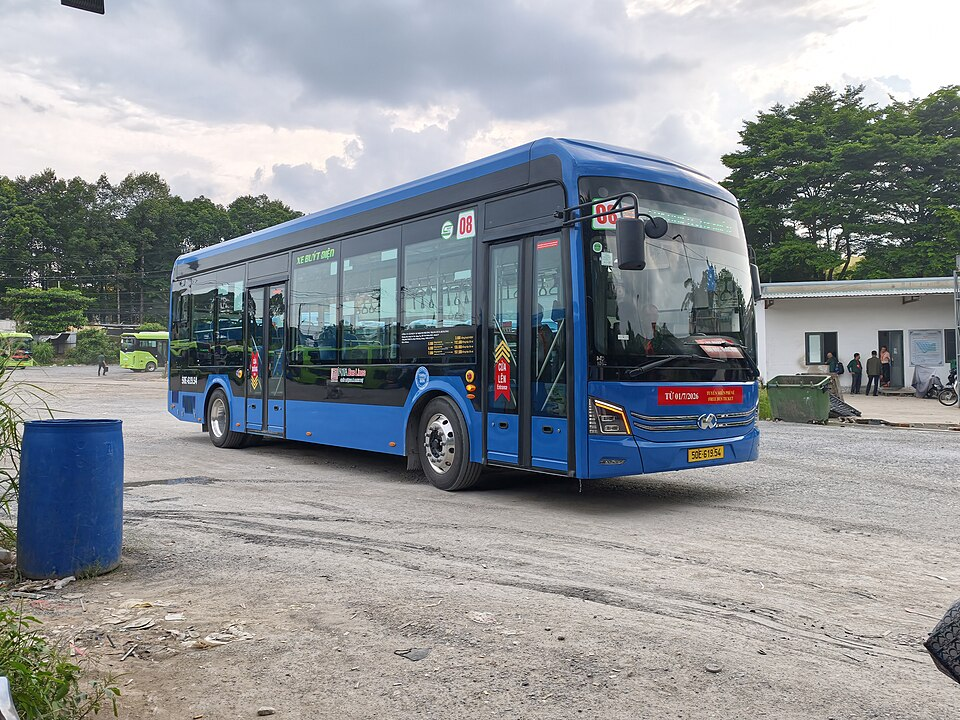
\includegraphics[width=\linewidth,height=0.55\textheight,keepaspectratio]{images/section-01/xe-buyt-tuyen-08.jpg}
      \\[0.15cm]
      {\scriptsize\color{gray!80!black}
        Xe buýt tuyến 08 (BX Quận 8 -- ĐHQG).\\
        Ảnh: Mrnhan16201, Wikimedia Commons\\
        (CC~BY-SA~4.0).%
      }
    \end{column}
  \end{columns}
\end{frame}

\begin{frame}{Từ xe đạp công cộng đến xe điện trong khu đô thị}
  \begin{columns}[T,onlytextwidth]
    \begin{column}{0.58\textwidth}
      \begin{block}{Mô hình đã có ở Việt Nam}
        Xe đạp công cộng nhận và trả theo trạm. Hà Nội và TP.HCM đã bổ sung xe đạp điện.
      \end{block}
      \vspace{0.15cm}
      \begin{block}{Đề xuất cho ĐHQG-HCM}
        Bố trí Hub xe điện dùng chung gần ký túc xá, trường học và điểm trung chuyển.
      \end{block}
      \vspace{0.25cm}
      \centering
      \begin{tikzpicture}[node distance=0.35cm]
        \node[key, font=\scriptsize, text width=2.45cm, minimum height=1.08cm] (s1) {Ký túc xá hoặc\\điểm trung chuyển};
        \node[key, font=\scriptsize, text width=2.05cm, minimum height=1.08cm, right=of s1] (s2) {Nhận xe\\tại Hub};
        \node[key, font=\scriptsize, text width=2.25cm, minimum height=1.08cm, right=of s2] (s3) {Trả xe tại Hub\\gần trường};
        \draw[arr, BKTemplate] (s1) -- (s2);
        \draw[arr, BKTemplate] (s2) -- (s3);
      \end{tikzpicture}
    \end{column}
    \begin{column}{0.39\textwidth}
      \centering
      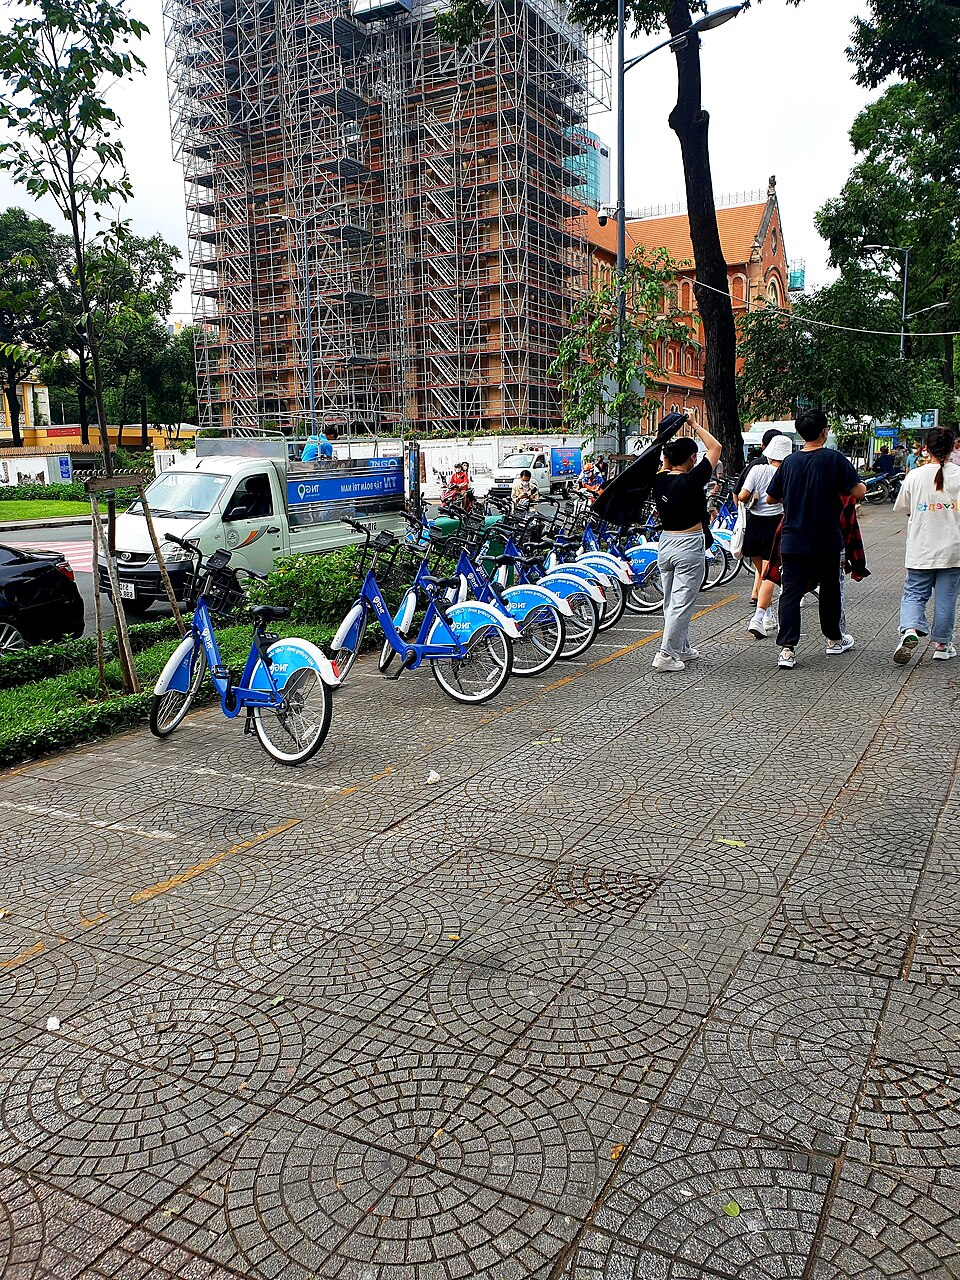
\includegraphics[width=\linewidth,height=0.55\textheight,keepaspectratio]{images/section-01/xe-dap-cong-cong-tngo.jpg}
      \\[0.15cm]
      {\scriptsize\color{gray!80!black}
        Xe đạp công cộng TNGo, Q.1, TP.HCM (2022).\\
        Ảnh: Phương Huy, Wikimedia Commons\\
        (CC0~1.0).%
      }
    \end{column}
  \end{columns}
\end{frame}

\begin{frame}{Mục tiêu của Smart E-Mobility Hub}
  \begin{columns}[T,onlytextwidth]
    \begin{column}{0.45\textwidth}
      \begin{block}{Sinh viên}
        Tìm xe còn trống, xem mức pin, giữ xe và kiểm tra chỗ trả.
      \end{block}
      \vspace{0.12cm}
      \begin{block}{Đơn vị vận hành}
        Theo dõi xe, chỗ đỗ và cổng sạc để điều chuyển xe và lập lịch sạc.
      \end{block}
      \vspace{0.12cm}
      \begin{block}{Mô phỏng What-if}
        Đánh giá khả năng phục vụ khi nhu cầu tăng trước khi quyết định điều phối.
      \end{block}
    \end{column}
    \begin{column}{0.52\textwidth}
      \centering
      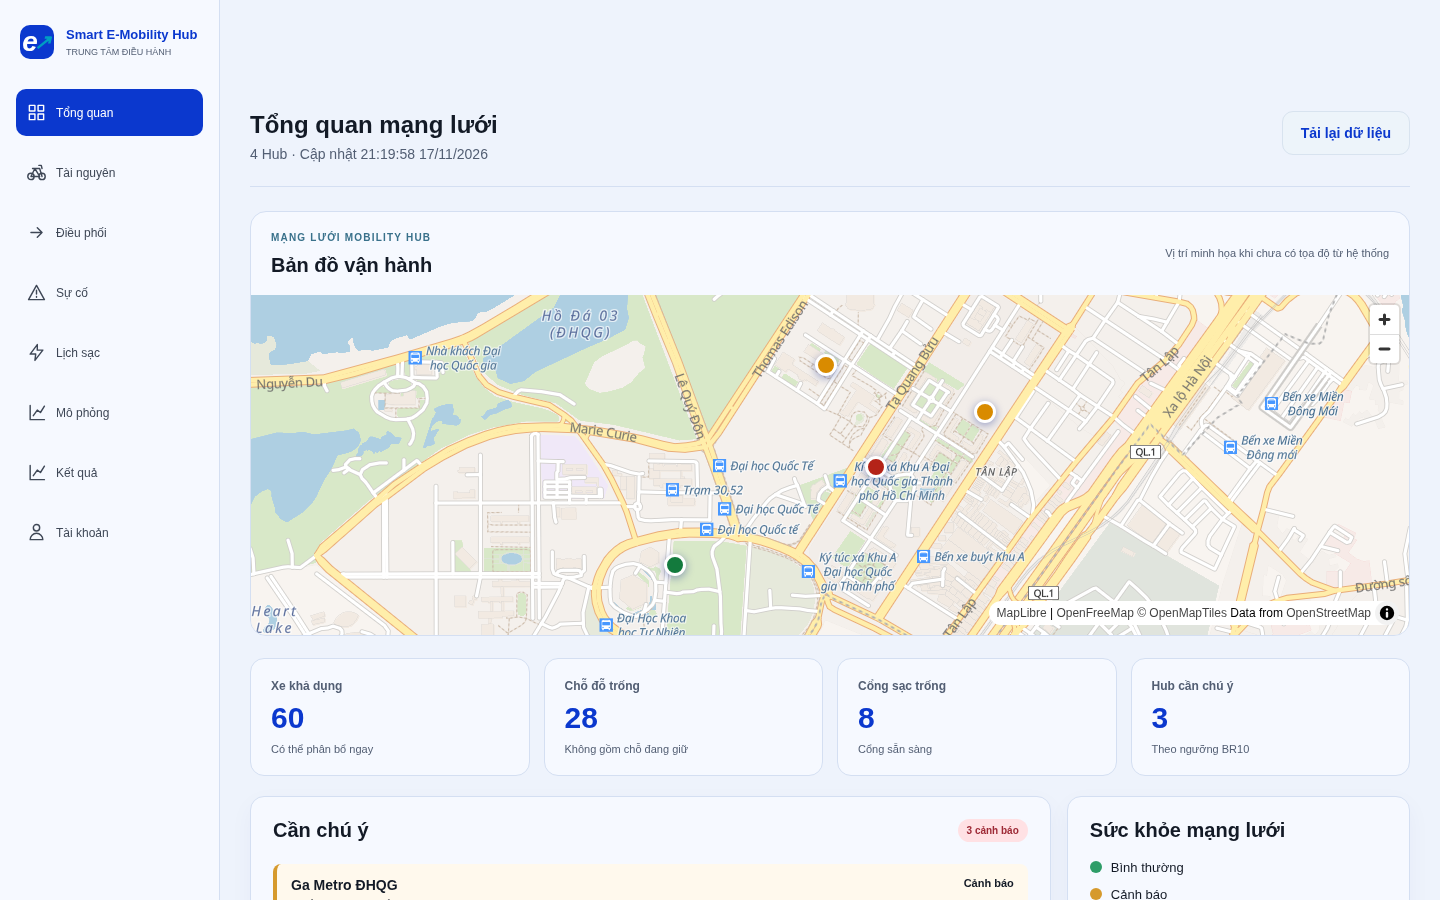
\includegraphics[width=\linewidth,height=0.60\textheight,keepaspectratio]{../../assets/demo/admin-overview.png}
      \\[0.18cm]
      {\scriptsize\color{gray!80!black}
        Bảng điều khiển mạng lưới Hub trong bản demo.\\
        Vị trí và số liệu trên màn hình dùng để minh họa.%
      }
    \end{column}
  \end{columns}
\end{frame}

\section{Yêu cầu và phạm vi ứng dụng}

\begin{frame}{Hệ thống cần đáp ứng những gì?}
  \centering
  \setlength{\tabcolsep}{6pt}
  {\small
  \begin{tabular}{@{}L{4.0cm}L{8.0cm}l@{}}
    \toprule
    \textbf{Nhóm yêu cầu} & \textbf{Chức năng} & \textbf{Use Case} \\
    \midrule
    \textbf{Thuê xe dùng chung} &
      Tìm Hub, xem xe và mức pin, giữ--nhận--trả xe &
      UC01--UC05 \\
    \addlinespace[6pt]
    \textbf{Đỗ và sạc xe cá nhân} &
      Đặt chỗ đỗ, ghi nhận xe vào/ra, gửi yêu cầu sạc &
      UC06--UC07 \\
    \addlinespace[6pt]
    \textbf{Vận hành mạng lưới} &
      Giám sát Hub, quản lý tài nguyên, điều chuyển xe, xử lý sự cố, lập lịch sạc &
      UC08--UC12 \\
    \addlinespace[6pt]
    \textbf{Mô phỏng What-if} &
      Chạy kịch bản giả định và xem kết quả &
      UC13--UC14 \\
    \bottomrule
  \end{tabular}
  }
  \vspace{0.35cm}
  \begin{tikzpicture}
    \node[key, text width=0.92\textwidth, align=left, inner sep=7pt] {%
      \textbf{Yêu cầu chất lượng:} Phân quyền theo vai trò, tránh cấp trùng xe hoặc chỗ đỗ, lưu dữ liệu nghiệp vụ qua lần khởi động lại.%
    };
  \end{tikzpicture}
\end{frame}

\begin{frame}{Sinh viên làm được gì trên Android?}
  \begin{columns}[T,onlytextwidth]
    \begin{column}{0.49\textwidth}
      \begin{block}{Xe dùng chung}
        Tìm Hub $\rightarrow$ xem xe và mức pin $\rightarrow$ giữ xe $\rightarrow$ nhận xe theo mã $\rightarrow$ chọn chỗ và trả xe.
      \end{block}
      \vspace{0.25cm}
      \begin{block}{Xe cá nhân}
        Đặt chỗ đỗ, check-in/check-out và gửi yêu cầu sạc.
      \end{block}
    \end{column}
    \begin{column}{0.48\textwidth}
      \begin{columns}[T,onlytextwidth]
        \begin{column}{0.48\textwidth}
          \centering
          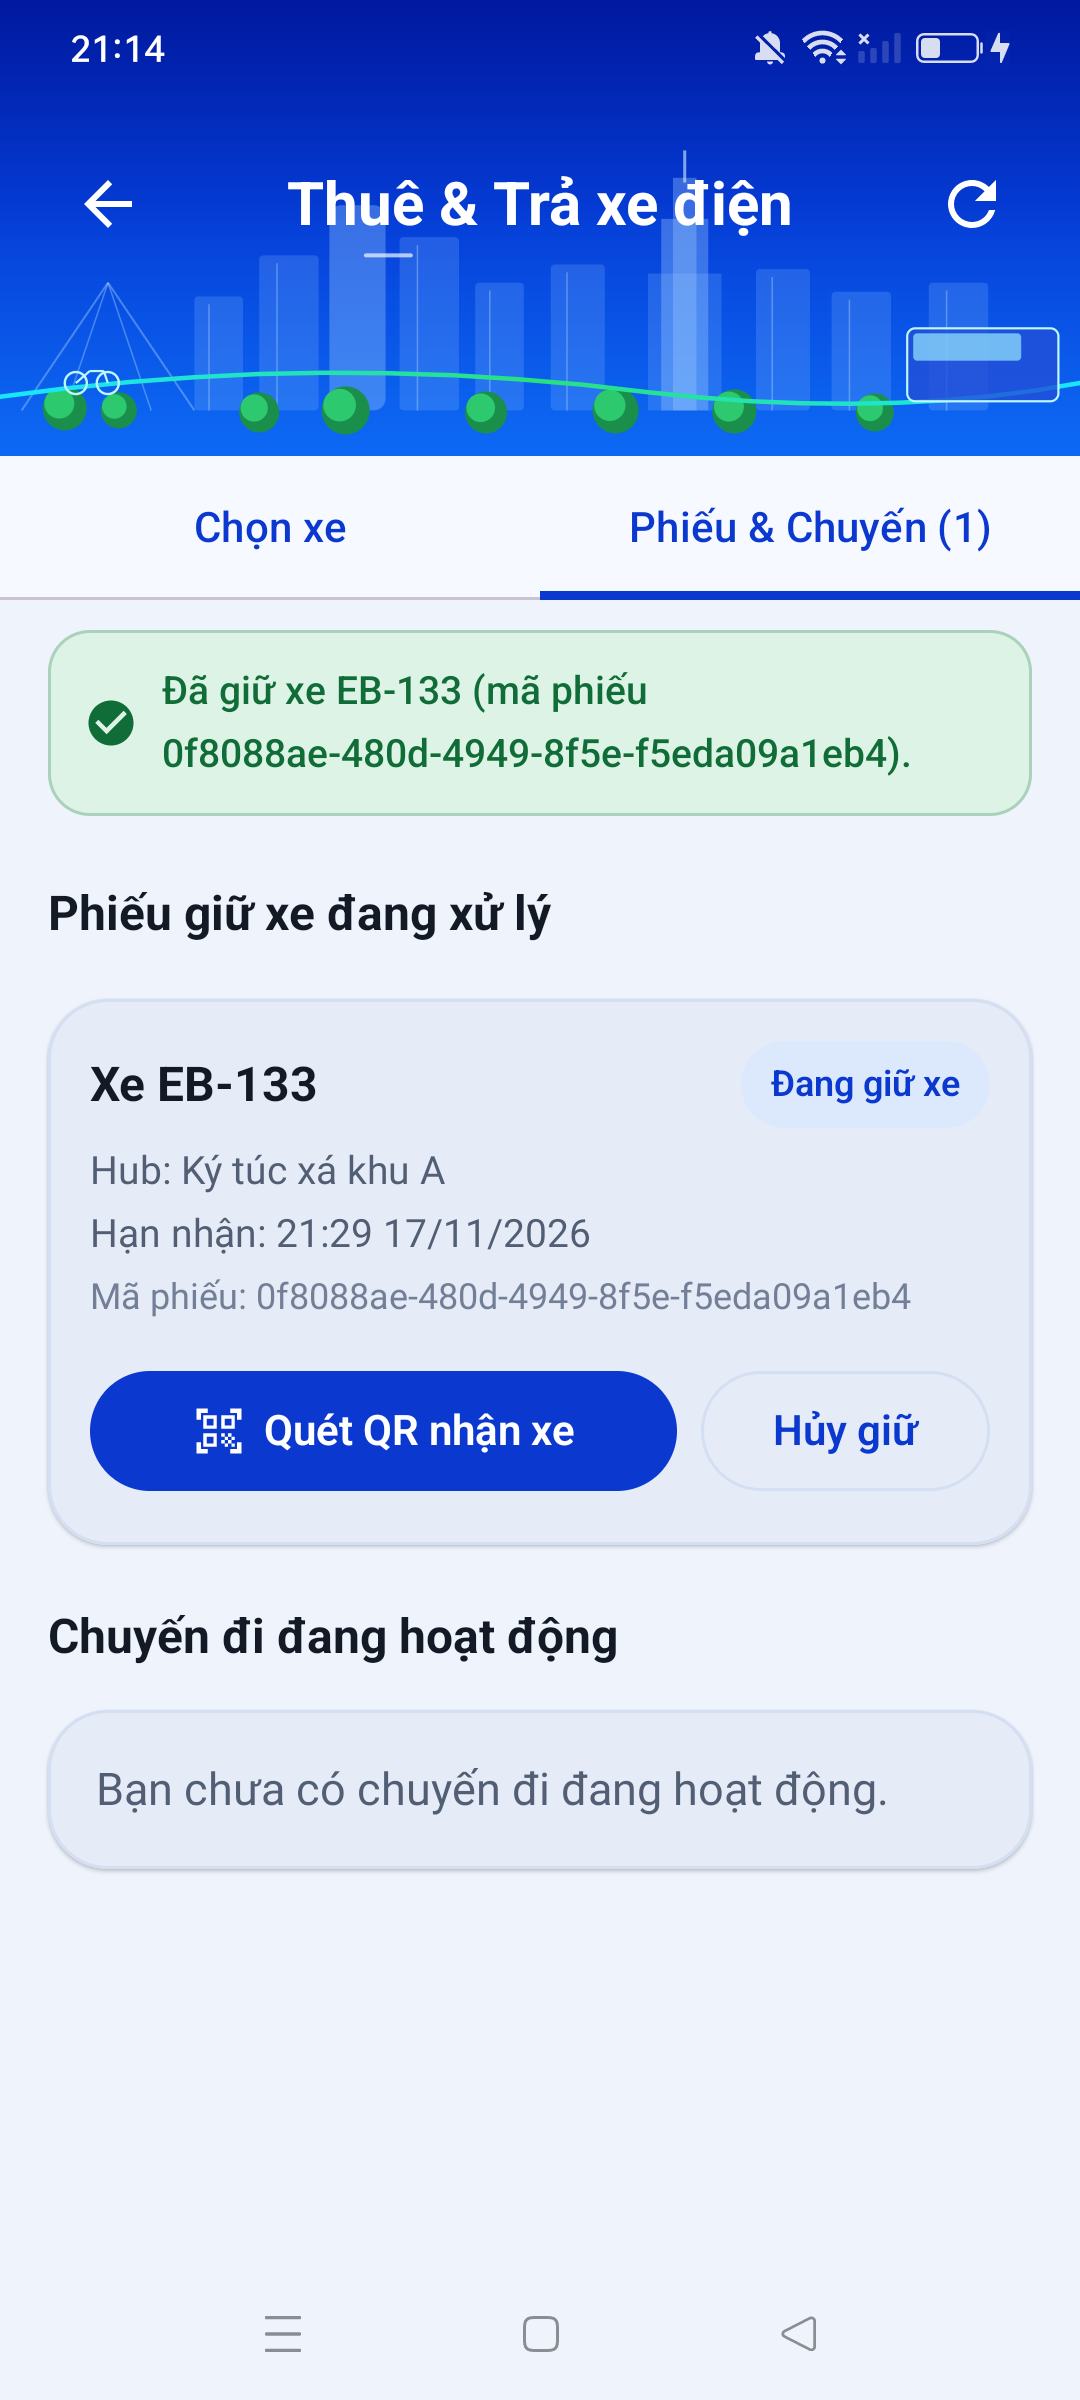
\includegraphics[width=\linewidth,height=0.58\textheight,keepaspectratio]{../../assets/demo/android-ticket.png}
          \\[0.12cm]
          {\scriptsize\color{gray!80!black} Phiếu giữ xe}
        \end{column}
        \begin{column}{0.48\textwidth}
          \centering
          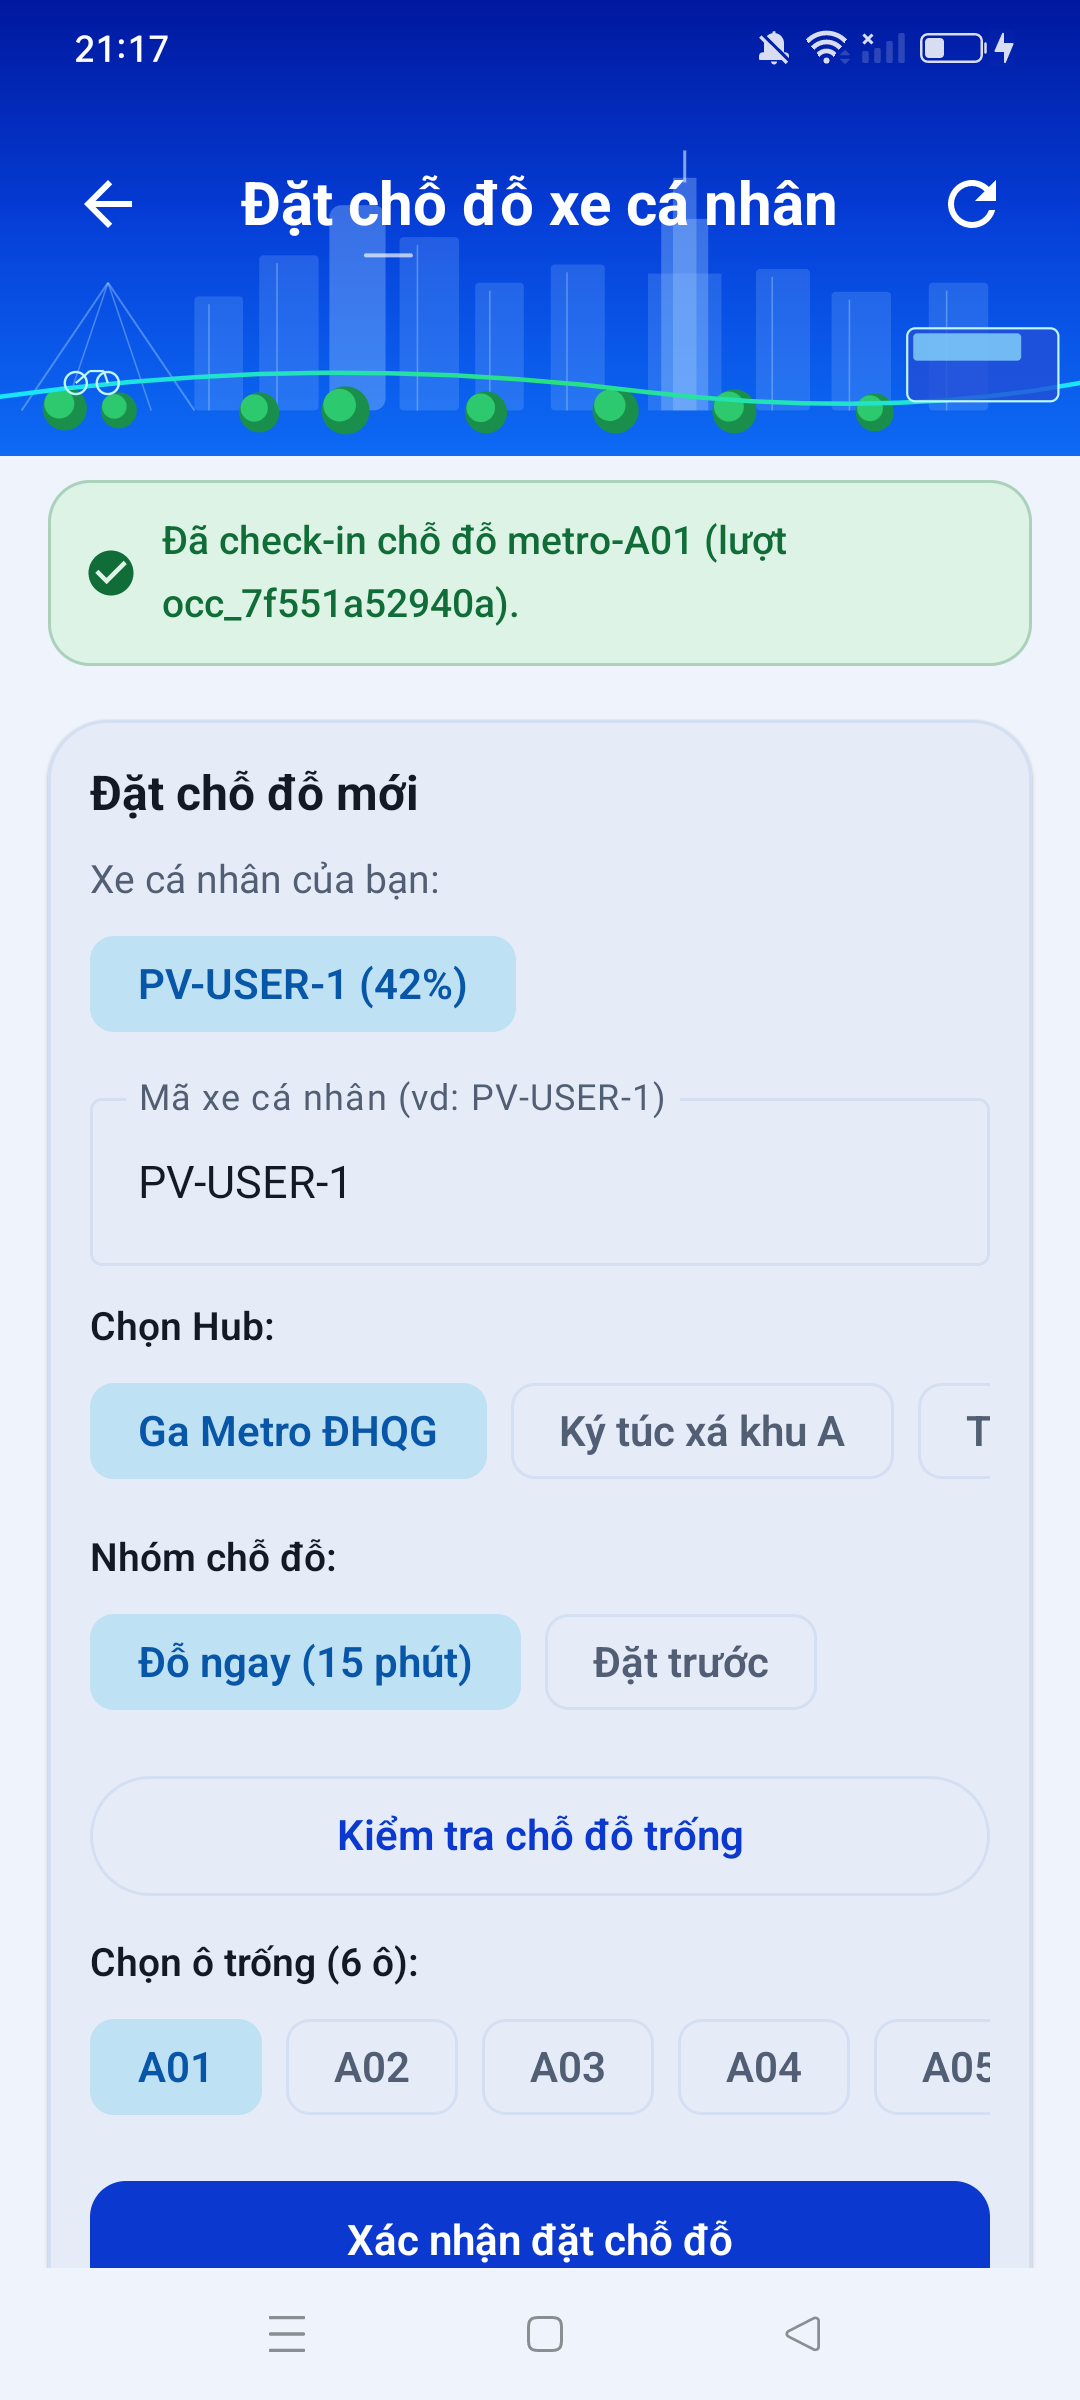
\includegraphics[width=\linewidth,height=0.58\textheight,keepaspectratio]{../../assets/demo/android-parking.png}
          \\[0.12cm]
          {\scriptsize\color{gray!80!black} Đặt chỗ đỗ xe cá nhân}
        \end{column}
      \end{columns}
    \end{column}
  \end{columns}
\end{frame}

\begin{frame}{Đơn vị vận hành làm được gì trên web?}
  \centering
  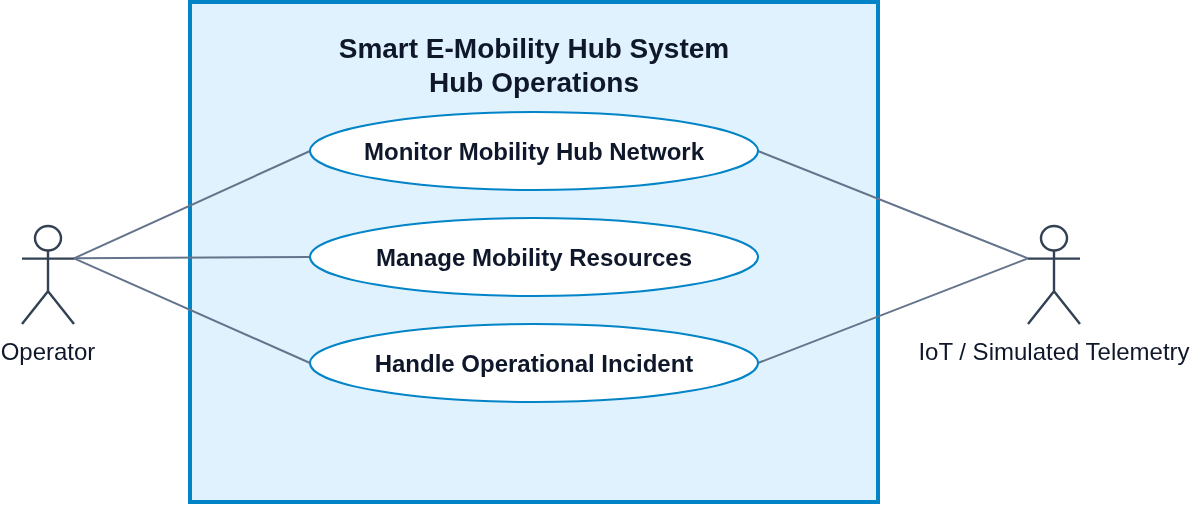
\includegraphics[width=0.78\textwidth,height=0.38\textheight,keepaspectratio]{images/section-02/workflow-hub-operations.png}
  \\[0.08cm]
  {\scriptsize\color{gray!80!black}
    Use Case vận hành Hub: giám sát mạng lưới, quản lý tài nguyên và xử lý sự cố.%
  }
  \vspace{0.18cm}
  \begin{columns}[T,onlytextwidth]
    \begin{column}{0.32\textwidth}
      \begin{block}{\footnotesize Giám sát, tài nguyên \& sự cố}
        \footnotesize Xem tình trạng Hub, quản lý xe, chỗ đỗ, cổng sạc và phân công bảo trì.
      \end{block}
    \end{column}
    \begin{column}{0.32\textwidth}
      \begin{block}{\footnotesize Điều chuyển xe}
        \footnotesize Lập lệnh giữa các Hub, xác nhận xe đến hoặc hủy lệnh theo trạng thái.
      \end{block}
    \end{column}
    \begin{column}{0.32\textwidth}
      \begin{block}{\footnotesize Lập lịch sạc}
        \footnotesize Xếp hàng theo ưu tiên và phân bổ cổng tương thích trong giới hạn công suất.
      \end{block}
    \end{column}
  \end{columns}
\end{frame}

\begin{frame}{What-if hỗ trợ quyết định như thế nào?}
  \begin{columns}[T,onlytextwidth]
    \begin{column}{0.53\textwidth}
      \centering
      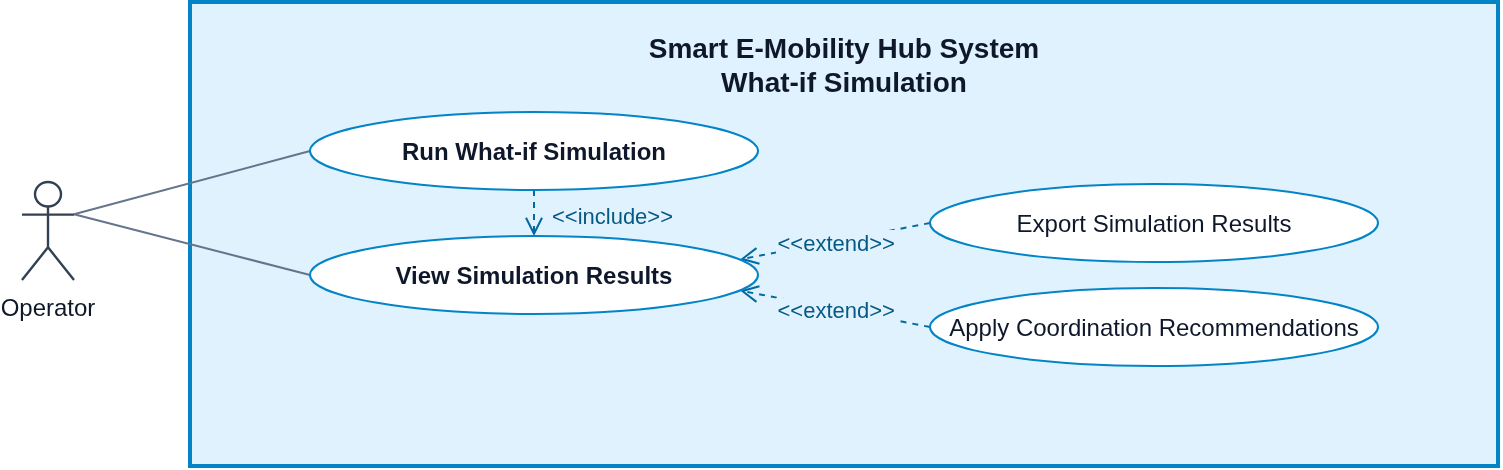
\includegraphics[width=\linewidth,height=0.34\textheight,keepaspectratio]{images/section-02/workflow-what-if-simulation.png}
      \vspace{0.18cm}
      \begin{block}{Luồng hỗ trợ quyết định}
        \footnotesize
        \begin{itemize}
          \setlength{\itemsep}{3pt}
          \item \textbf{Chạy kịch bản:} Chọn tình huống giả định, chẳng hạn khách đến ga Metro tăng đột biến.
          \item \textbf{Đọc kết quả:} So sánh tỷ lệ phục vụ và thời gian chờ giữa cơ sở và kịch bản.
          \item \textbf{Xem phương án:} Mở khuyến nghị điều chuyển và xác nhận tạo lệnh riêng khi cần.
        \end{itemize}
      \end{block}
    \end{column}
    \begin{column}{0.44\textwidth}
      \centering
      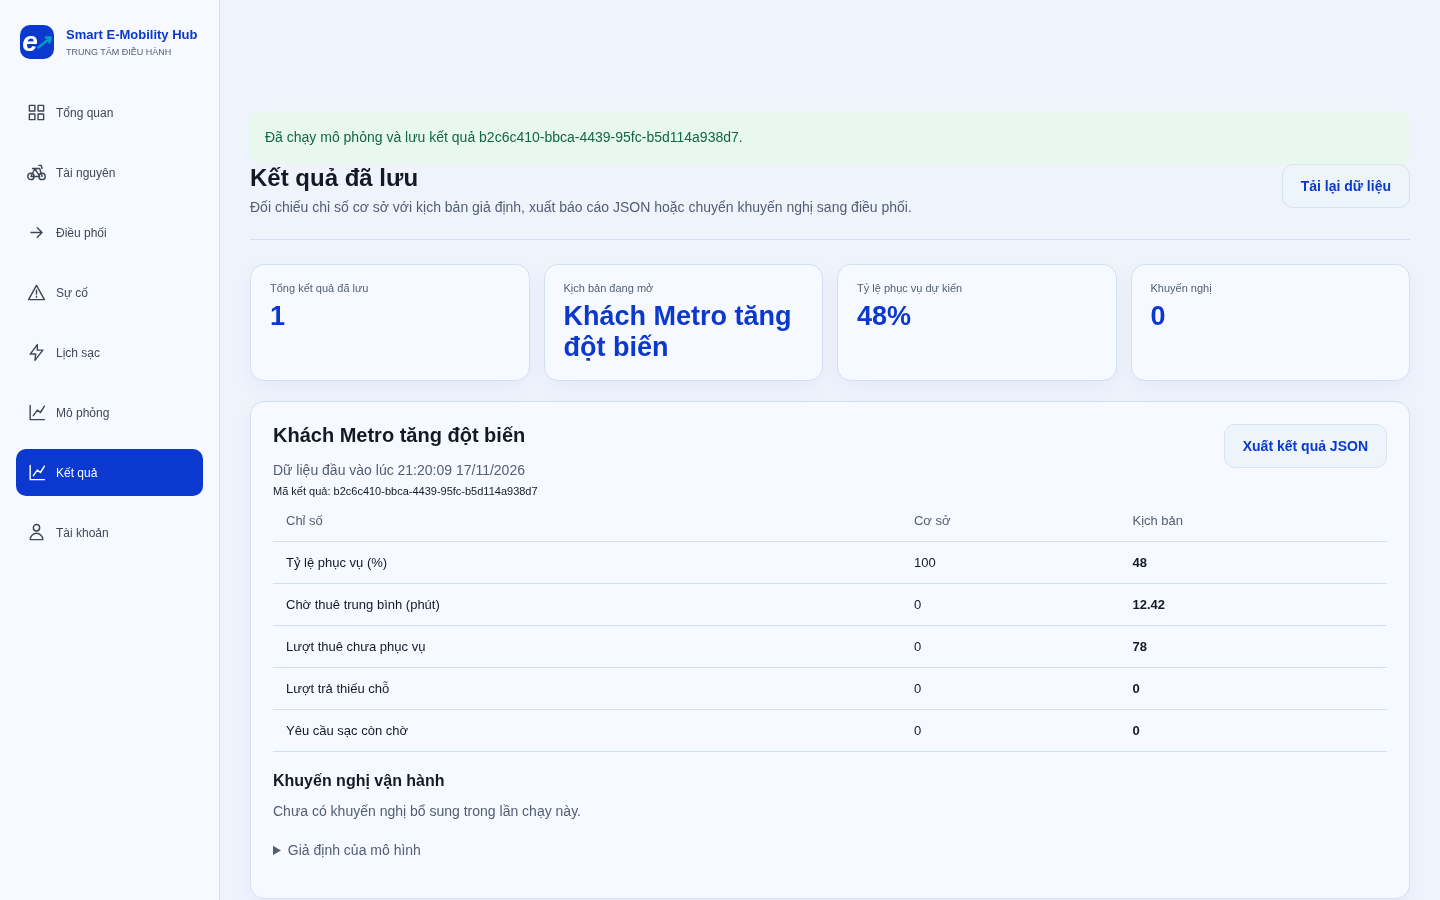
\includegraphics[width=\linewidth,height=0.60\textheight,keepaspectratio]{../../assets/demo/admin-simulation.png}
      \\[0.15cm]
      {\scriptsize\color{gray!80!black}
        Kết quả của một lượt chạy với dữ liệu demo.%
      }
    \end{column}
  \end{columns}
\end{frame}

\begin{frame}{MVP đã triển khai đến đâu?}
  \centering
  \setlength{\tabcolsep}{6pt}
  {\small
  \begin{tabular}{@{}L{3.6cm}L{10.4cm}@{}}
    \toprule
    \textbf{Phạm vi} & \textbf{Trạng thái} \\
    \midrule
    \textbf{Đã có trong demo} &
      Luồng thuê xe, đỗ và gửi yêu cầu sạc trên Android. Giám sát, quản lý tài nguyên, điều chuyển, xử lý sự cố, lập lịch sạc và What-if trên web. Xác nhận thiết bị dùng dữ liệu giả lập. \\
    \addlinespace[8pt]
    \textbf{Còn giới hạn} &
      Kích hoạt phiên sạc, xác nhận tháo kết nối và xác minh cách ly thiết bị có xử lý ở tầng dịch vụ. Tích hợp IoT thật và gửi thông báo qua dịch vụ ngoài chưa được triển khai. \\
    \addlinespace[8pt]
    \textbf{Ngoài phạm vi MVP} &
      Đăng ký tự phục vụ, thanh toán và ứng dụng riêng cho kỹ thuật viên. Tài khoản và xe cá nhân được cấp sẵn để trình diễn. \\
    \bottomrule
  \end{tabular}
  }
\end{frame}

\section{Thiết kế nghiệp vụ và giao diện}

\begin{frame}{Thiết kế qua hai phiên bản}
  \centering
  \setlength{\tabcolsep}{6pt}
  {\small
  \begin{tabular}{@{}L{3.35cm}L{10.35cm}@{}}
    \toprule
    \textbf{Giai đoạn} & \textbf{Nội dung} \\
    \midrule
    \textbf{Version 1} &
      Đặc tả ban đầu, Use Case và prototype để thống nhất phạm vi và luồng thao tác. \\
    \addlinespace[8pt]
    \textbf{Qua các buổi họp} &
      Rà soát tiến độ, thảo luận thay đổi về luồng và ngoại lệ, rồi cập nhật đặc tả, UML và giao diện. \\
    \addlinespace[8pt]
    \textbf{Version 2 · Bản trình bày} &
      Làm rõ quy tắc giữ, nhận và trả xe; đối chiếu lại yêu cầu và UML với các luồng chạy trên Android và web. \\
    \bottomrule
  \end{tabular}
  }
  \vspace{0.42cm}
  \begin{tikzpicture}
    \node[key, text width=0.91\textwidth, align=left, inner sep=7pt] {%
      \textbf{Ví dụ xuyên suốt:} Giữ xe tạo một phiếu có hạn; chuyến đi chỉ bắt đầu sau khi dock xác nhận mở khóa.%
    };
  \end{tikzpicture}
\end{frame}

\begin{frame}{Activity Diagram — Khi nào giữ xe thành công?}
  \begin{columns}[T,onlytextwidth]
    \begin{column}{0.37\textwidth}
      \centering
      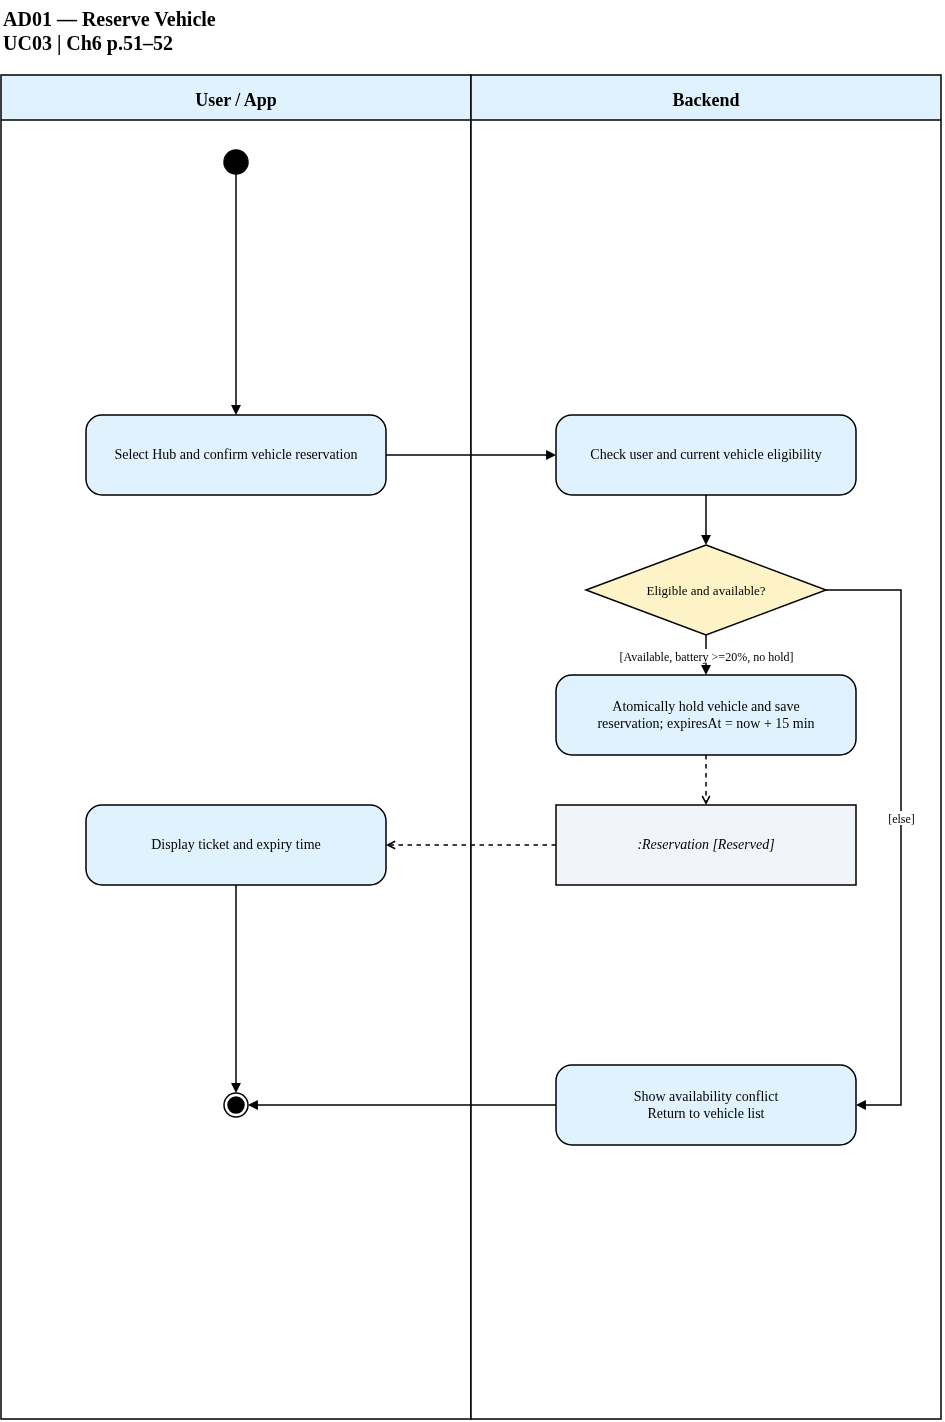
\includegraphics[width=\linewidth,height=0.64\textheight,keepaspectratio]{images/section-03/ad01-giu-xe.png}
      \\[0.08cm]
      {\scriptsize\color{gray!80!black} AD01 · Đặt giữ xe}
    \end{column}
    \begin{column}{0.60\textwidth}
      \small
      \begin{block}{UC03 · Luồng chính}
        Chọn xe $\rightarrow$ kiểm tra khả dụng $\rightarrow$ giữ xe và tạo phiếu 15 phút.
      \end{block}
      \vspace{0.08cm}
      \begin{block}{Xe đủ điều kiện}
        Hệ thống giữ xe và lưu phiếu trong \textbf{cùng một giao dịch}; thời hạn được tính tại máy chủ.
      \end{block}
      \vspace{0.08cm}
      \begin{alertblock}{Xe không còn khả dụng}
        Ứng dụng báo xung đột và quay lại danh sách để sinh viên chọn xe khác.
      \end{alertblock}
    \end{column}
  \end{columns}
\end{frame}

\begin{frame}{Sequence Diagram — Ai xác nhận việc nhận xe?}
  \centering
  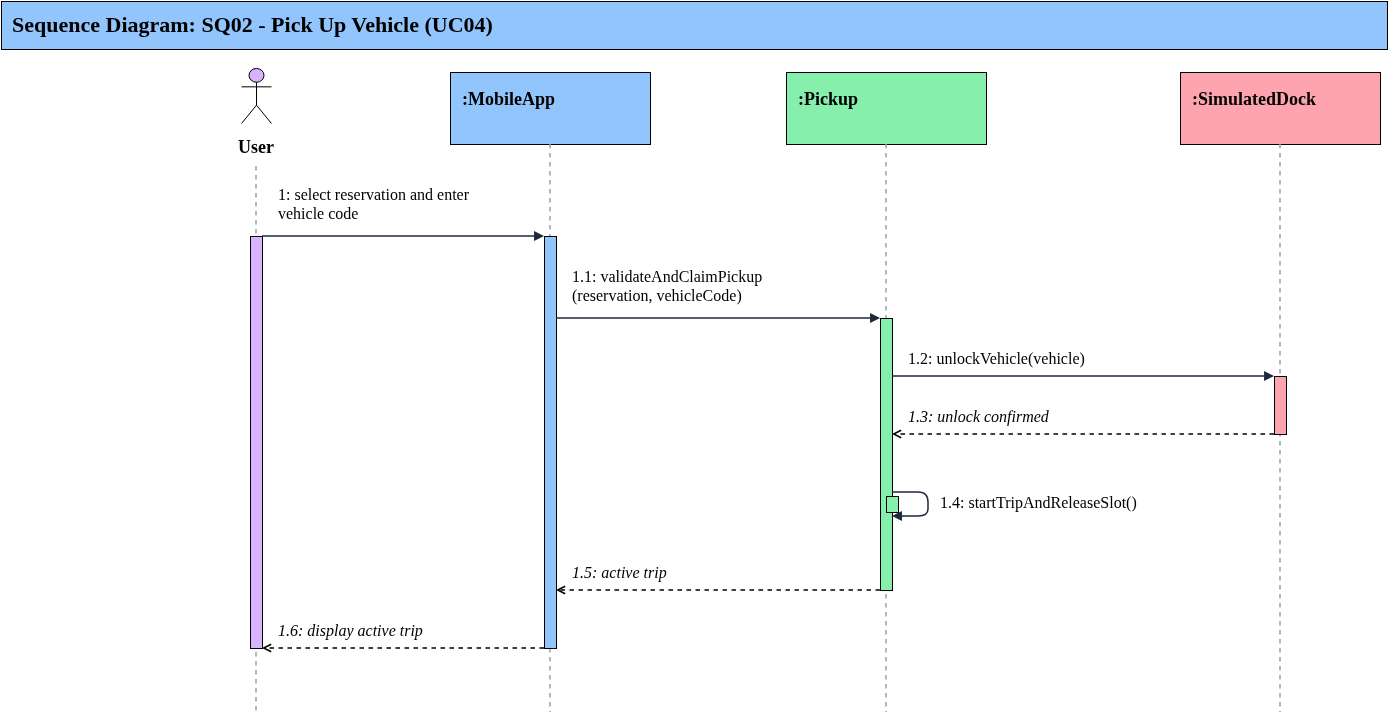
\includegraphics[width=0.91\textwidth,height=0.45\textheight,keepaspectratio]{images/section-03/sq02-nhan-xe.png}
  \vspace{0.12cm}
  \begin{tikzpicture}
    \node[key, text width=0.91\textwidth, align=left, inner sep=6pt] {%
      \textbf{UC04:} Sinh viên gửi mã xe $\rightarrow$ Mobile App chuyển yêu cầu $\rightarrow$ backend kiểm tra phiếu $\rightarrow$ dock giả lập xác nhận mở khóa $\rightarrow$ hệ thống bắt đầu chuyến và giải phóng chỗ đỗ.\\[3pt]
      \textbf{Ngoại lệ:} Nếu kết quả mở khóa chưa rõ, hệ thống giữ quyền nhận xe để đối soát thay vì tự giải phóng tài nguyên.%
    };
  \end{tikzpicture}
\end{frame}

\begin{frame}{State-chart — Xe đổi trạng thái khi nào?}
  \centering
  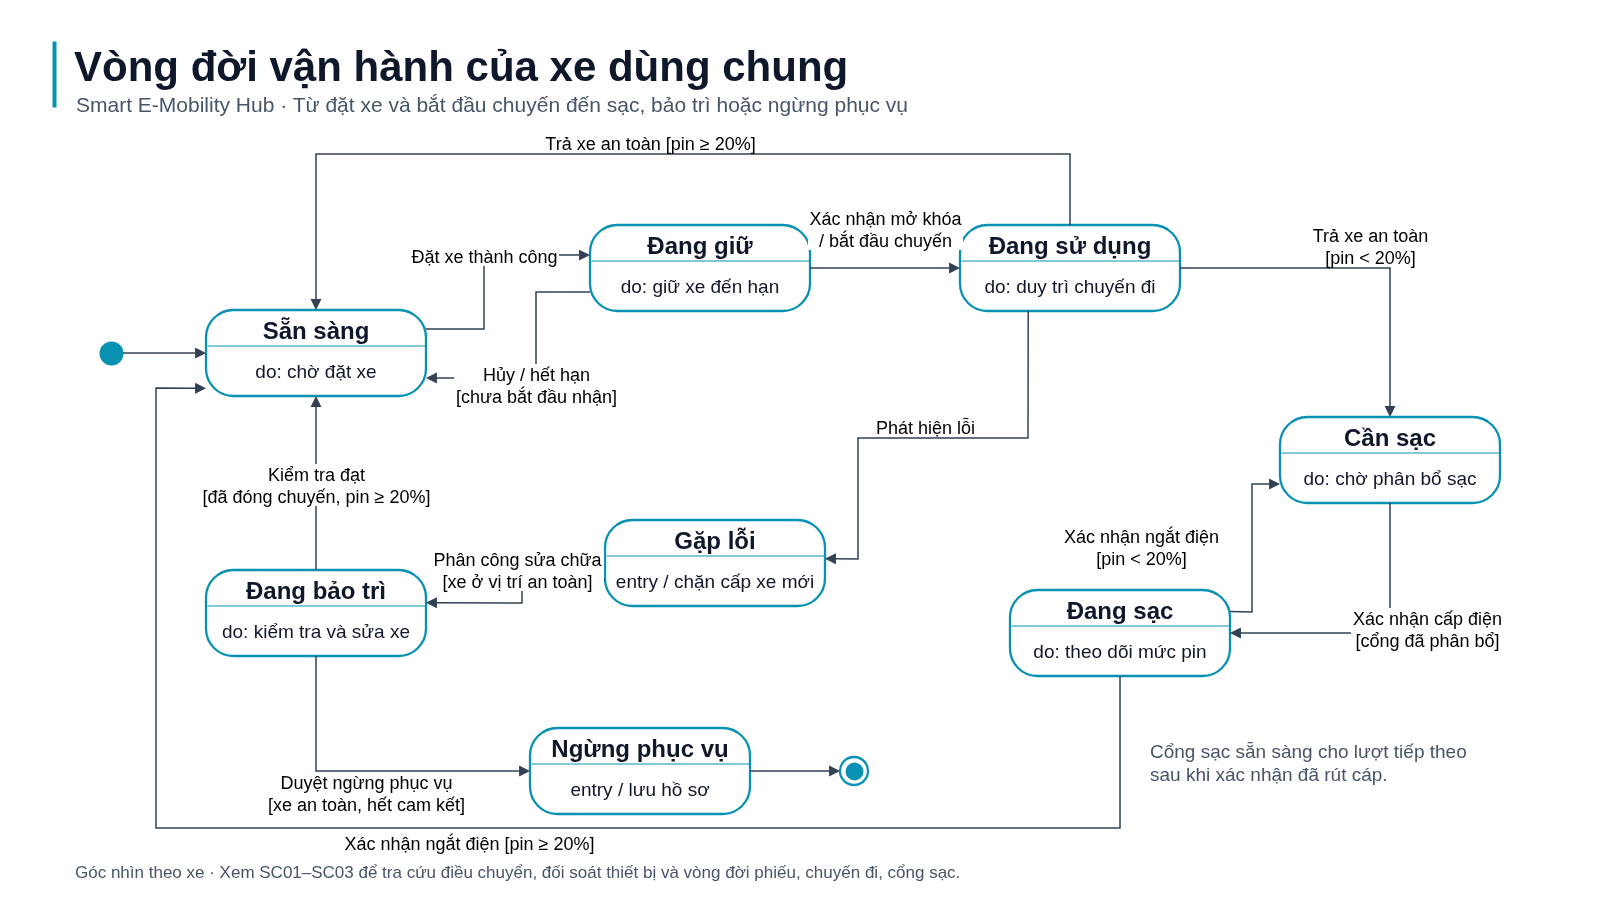
\includegraphics[width=0.90\textwidth,height=0.58\textheight,keepaspectratio]{images/section-03/sc00-vong-doi-xe.png}
  \vspace{0.12cm}
  \begin{columns}[T,onlytextwidth]
    \begin{column}{0.48\textwidth}
      \begin{block}{\footnotesize Trước chuyến đi}
        \footnotesize \textbf{Sẵn sàng $\rightarrow$ Đang giữ $\rightarrow$ Đang sử dụng} khi giữ xe thành công và dock xác nhận mở khóa.
      \end{block}
    \end{column}
    \begin{column}{0.49\textwidth}
      \begin{block}{\footnotesize Sau khi trả xe}
        \footnotesize Xe về \textbf{Sẵn sàng} nếu pin $\geq 20\%$, hoặc chuyển sang \textbf{Cần sạc} nếu pin $<20\%$.
      \end{block}
    \end{column}
  \end{columns}
\end{frame}

\begin{frame}{Từ mô hình lớp đến màn hình Android}
  \begin{columns}[T,onlytextwidth]
    \begin{column}{0.67\textwidth}
      \centering
      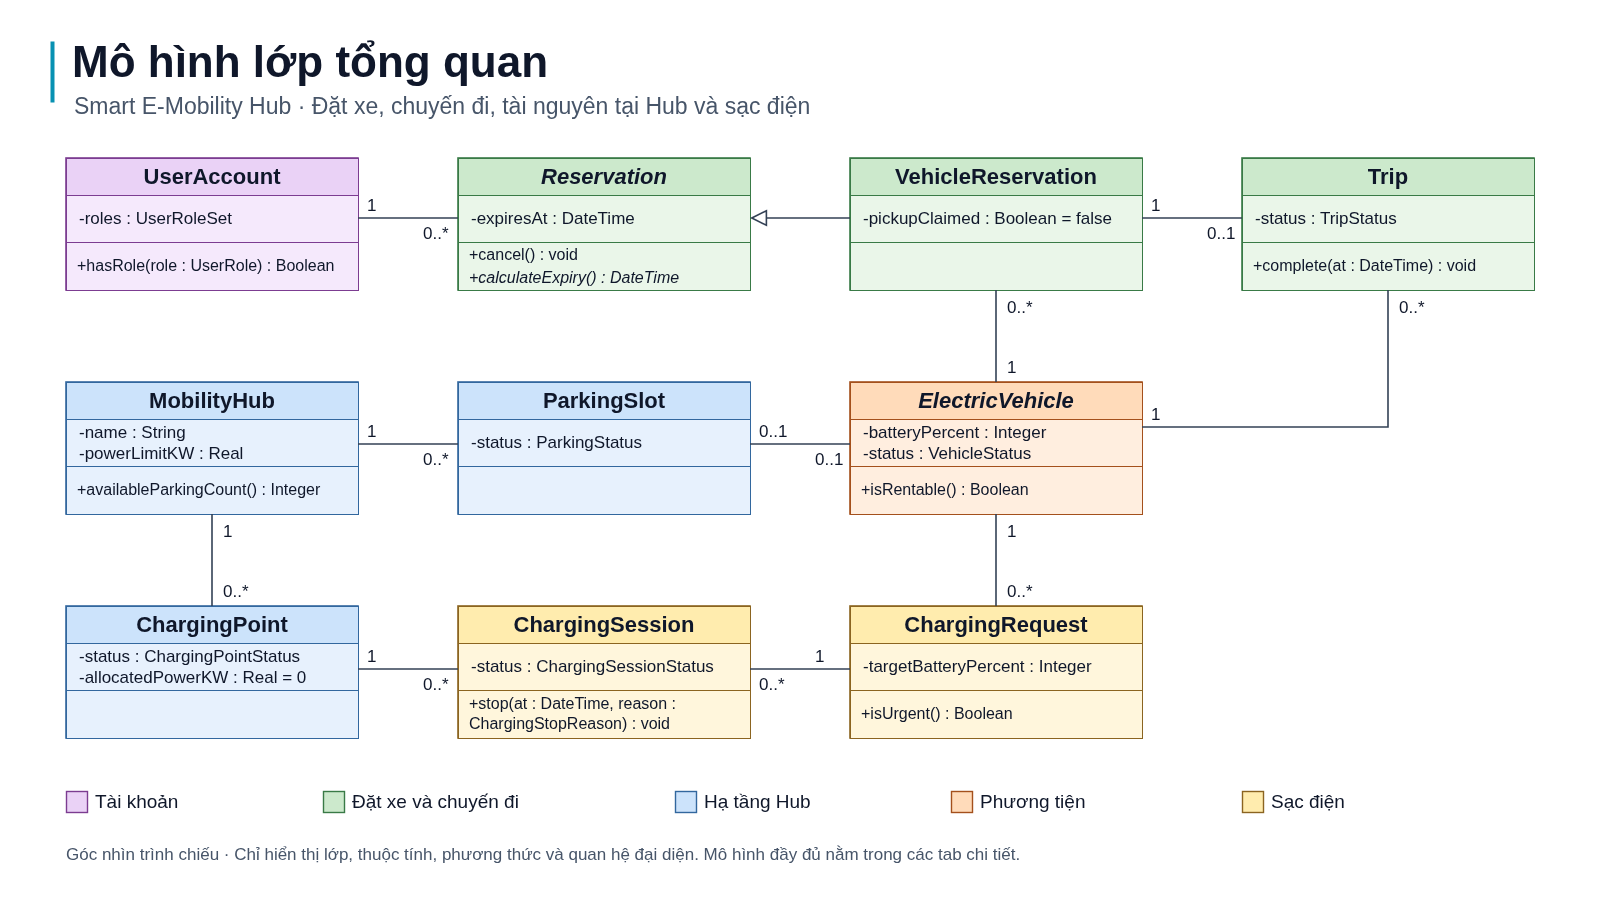
\includegraphics[width=\linewidth,height=0.54\textheight,keepaspectratio]{images/section-03/cd00-mo-hinh-lop.png}
      \\[0.06cm]
      {\scriptsize\color{gray!80!black}
        VehicleReservation liên kết người dùng, xe và tối đa một Trip.%
      }
    \end{column}
    \begin{column}{0.30\textwidth}
      \begin{block}{\footnotesize Phiếu giữ xe}
        \scriptsize \textbf{VehicleReservation}: mã xe, hạn nhận và trạng thái xác nhận.
      \end{block}
      \begin{block}{\footnotesize Chuyến đi}
        \scriptsize \textbf{Trip}: trạng thái sau khi nhận xe và thao tác trả xe.
      \end{block}
      \begin{block}{\footnotesize Tài nguyên Hub}
        \scriptsize \textbf{ElectricVehicle, ParkingSlot}: mức pin, xe khả dụng và chỗ có thể trả.
      \end{block}
      \centering
      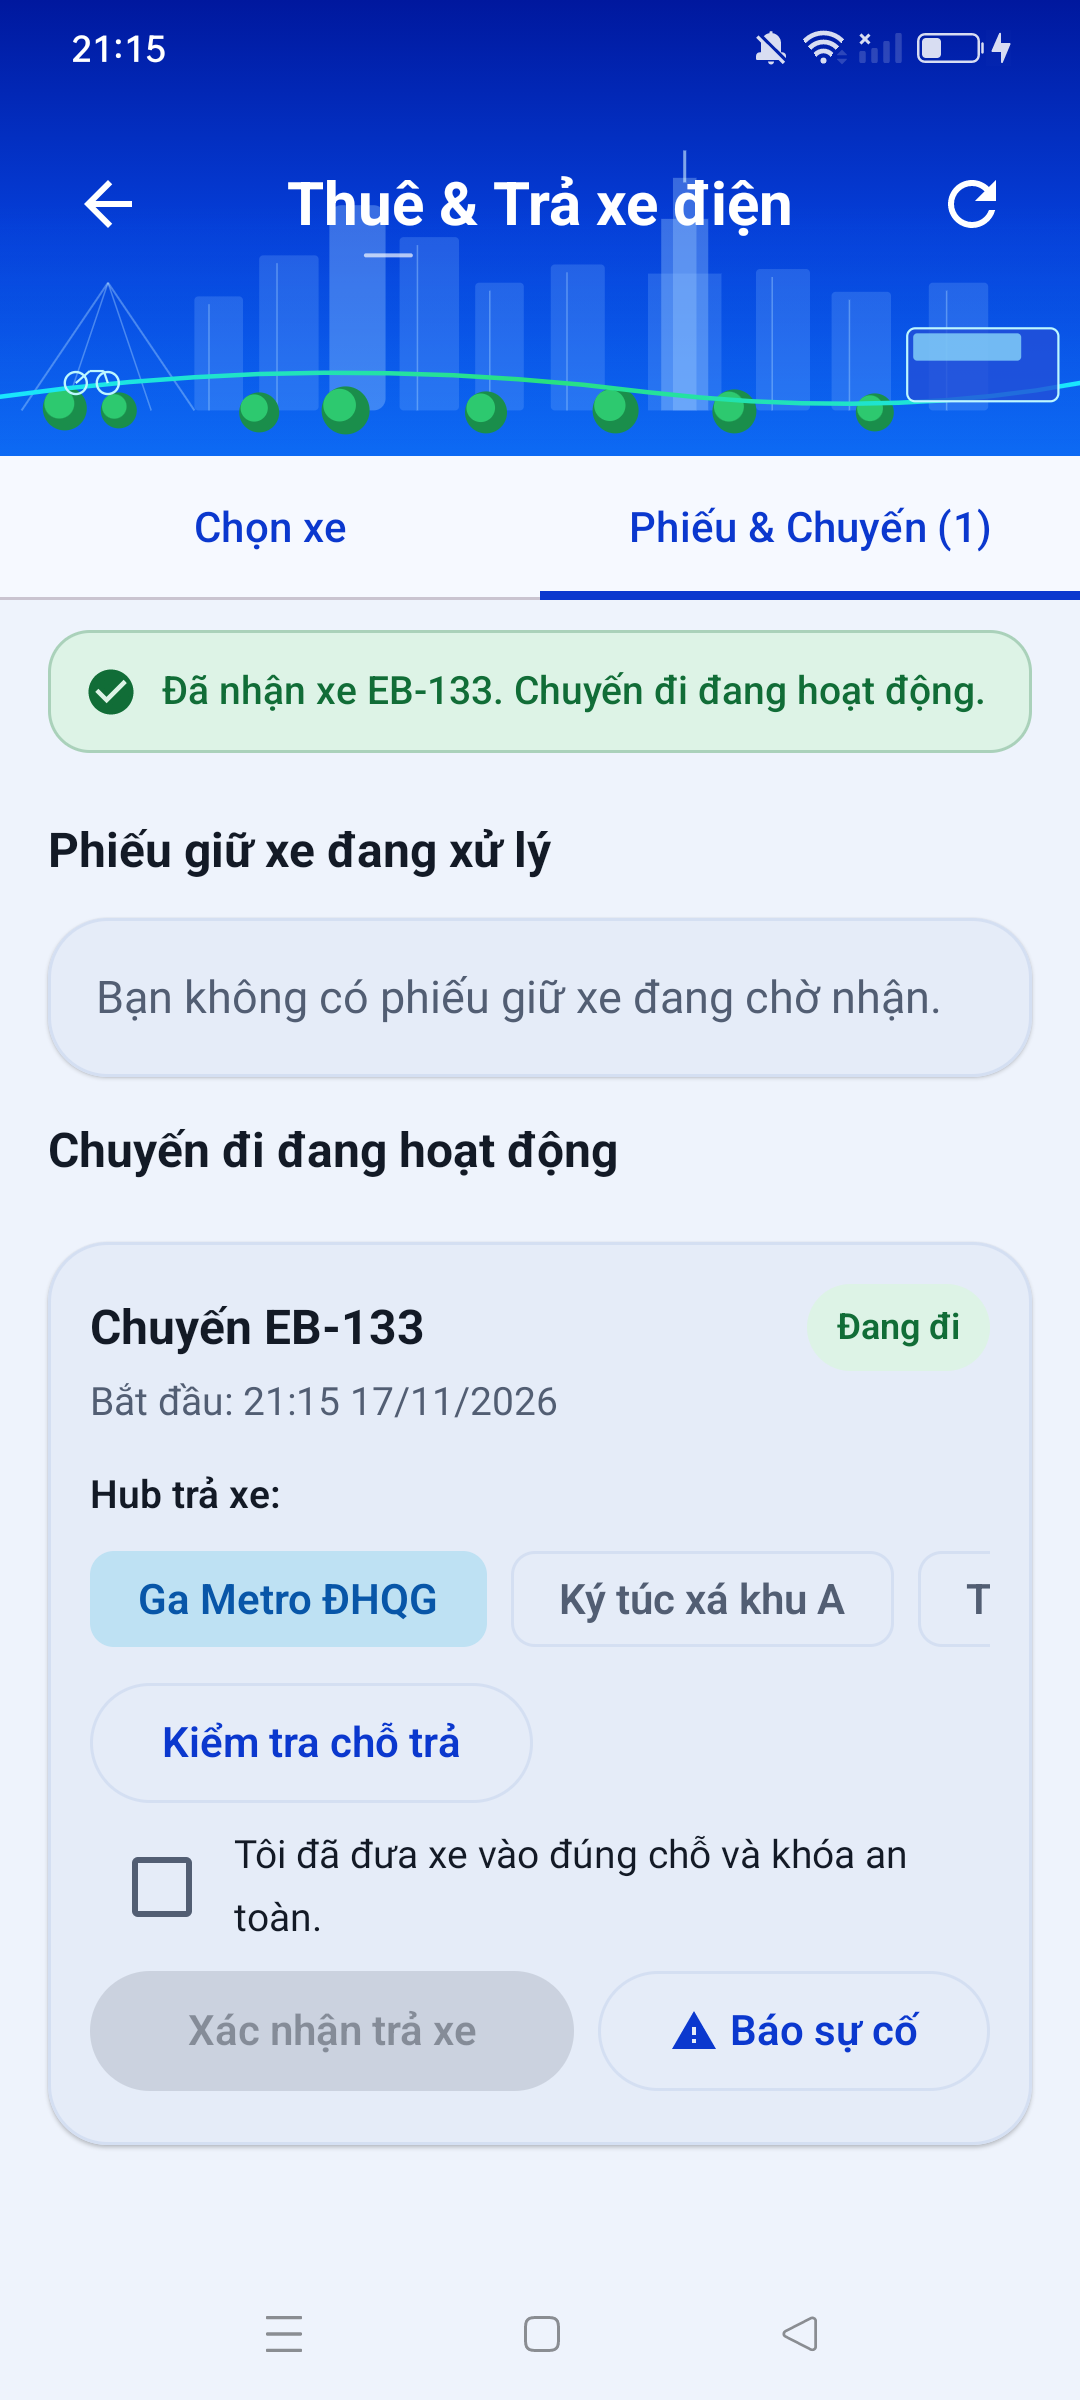
\includegraphics[width=0.52\linewidth,height=0.17\textheight,keepaspectratio]{../../assets/demo/android-active-trip.png}
    \end{column}
  \end{columns}
\end{frame}

\section{Kiến trúc và hiện thực MVP}

\begin{frame}{Một backend, ba module nghiệp vụ}
  \begin{columns}[T,onlytextwidth]
    \begin{column}{0.43\textwidth}
      \begin{block}{Kiến trúc MVP}
        Một ứng dụng \textbf{Node.js/Express} tổ chức theo \textbf{modular monolith}.
      \end{block}
      \vspace{0.2cm}
      \begin{block}{Lý do lựa chọn}
        Một backend dễ lắp ghép cho demo. Các luồng liên quan có thể dùng chung giao dịch khi cập nhật tài nguyên vật lý.
      \end{block}
      \vspace{0.25cm}
      \begin{tikzpicture}
        \node[key, text width=0.88\linewidth, align=left, inner sep=7pt] {%
          \textbf{Nguyên tắc:} module tách trách nhiệm nghiệp vụ, nhưng cùng được triển khai như một ứng dụng.%
        };
      \end{tikzpicture}
    \end{column}
    \begin{column}{0.54\textwidth}
      \begin{block}{Mobility / Simulation}
        Giữ–nhận–trả xe, quản lý chuyến đi và mô phỏng What-if.
      \end{block}
      \begin{block}{Operations}
        Quản lý tài nguyên, giám sát Hub, điều chuyển và xử lý sự cố.
      \end{block}
      \begin{block}{Parking / Charging}
        Đặt chỗ đỗ, ghi nhận xe vào/ra, yêu cầu và lập lịch sạc.
      \end{block}
    \end{column}
  \end{columns}
\end{frame}

\begin{frame}{Development View — Mã nguồn được chia thế nào?}
  \begin{columns}[T,onlytextwidth]
    \begin{column}{0.68\textwidth}
      \centering
      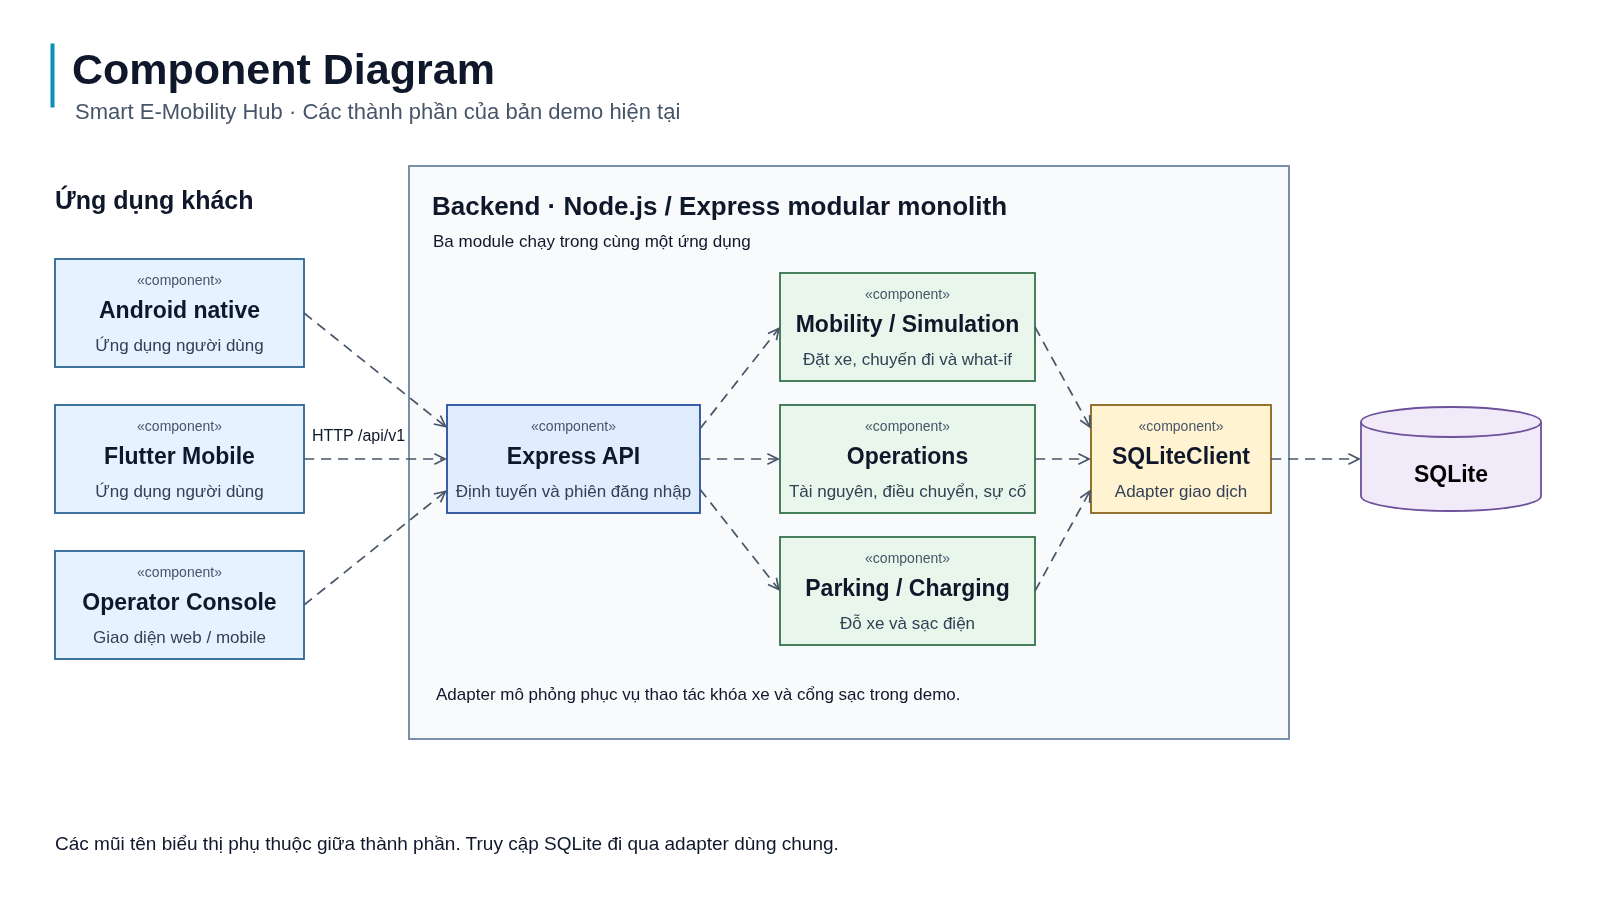
\includegraphics[width=\linewidth,height=0.62\textheight,keepaspectratio]{images/section-04/dv01-component-mvp.png}
    \end{column}
    \begin{column}{0.29\textwidth}
      \begin{block}{\footnotesize Thiết kế mục tiêu}
        \scriptsize Năm tầng: Presentation, API / Interface, Application, Domain và Infrastructure.
      \end{block}
      \vspace{0.06cm}
      \begin{block}{\footnotesize Version 2 đang chạy}
        \scriptsize Một Express app lắp ghép ba module. Các module truy cập dữ liệu qua repository và SQLiteClient dùng chung.
      \end{block}
      \vspace{0.06cm}
      \begin{block}{\footnotesize Ranh giới tích hợp}
        \scriptsize Mobility và Parking gọi giao diện quản lý tài nguyên do Operations cung cấp; thiết bị thật được thay bằng adapter mô phỏng.
      \end{block}
    \end{column}
  \end{columns}
\end{frame}

\begin{frame}{Physical View — Demo chạy ở đâu?}
  \begin{columns}[T,onlytextwidth]
    \begin{column}{0.60\textwidth}
      \centering
      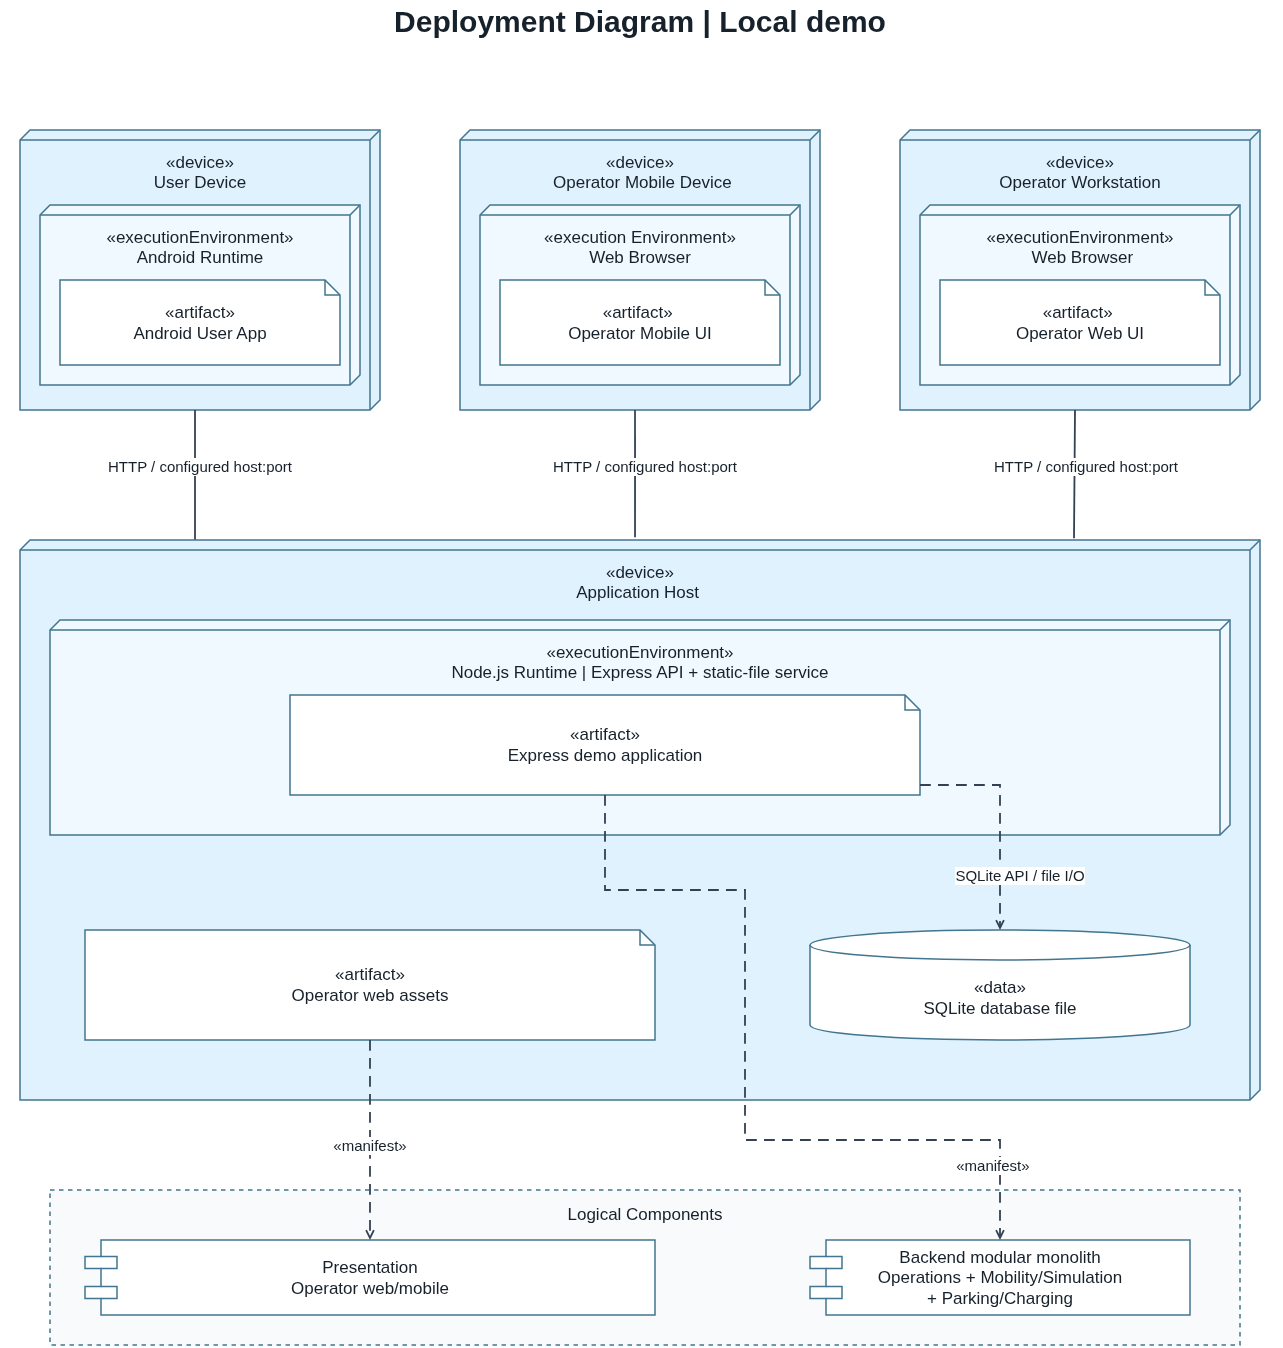
\includegraphics[width=\linewidth,height=0.63\textheight,keepaspectratio]{images/section-04/dp01-trien-khai-demo.png}
    \end{column}
    \begin{column}{0.37\textwidth}
      \begin{block}{\footnotesize Thiết bị Android}
        \footnotesize Ứng dụng sinh viên chạy trên thiết bị hoặc emulator.
      \end{block}
      \begin{block}{\footnotesize Trình duyệt}
        \footnotesize Giao diện Operator chạy trên web desktop hoặc mobile.
      \end{block}
      \begin{block}{\footnotesize Máy chạy demo}
        \footnotesize Node.js/Express phục vụ API và web assets; tệp SQLite nằm trên cùng máy.
      \end{block}
      {\scriptsize\textbf{Kết nối:} cùng một host HTTP trong cấu hình demo cục bộ.}
    \end{column}
  \end{columns}
\end{frame}

\begin{frame}{UC05 — Theo dấu một yêu cầu trả xe}
  \begin{columns}[T,onlytextwidth]
    \begin{column}{0.58\textwidth}
      \centering
      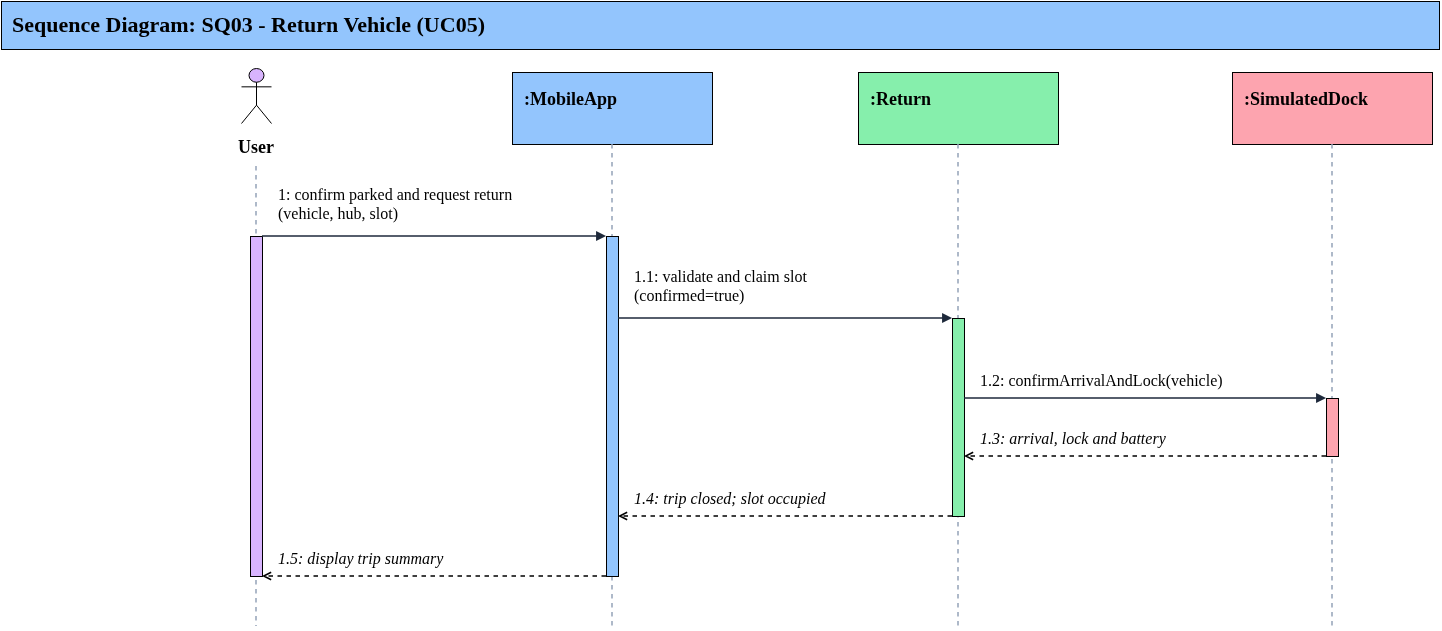
\includegraphics[width=\linewidth,height=0.57\textheight,keepaspectratio]{images/section-04/sq03-tra-xe.png}
      \\[0.12cm]
      {\scriptsize\color{gray!80!black} SQ03 · Trả xe dùng chung}
    \end{column}
    \begin{column}{0.39\textwidth}
      \small
      \begin{enumerate}
        \setlength{\itemsep}{6pt}
        \item \textbf{Android:} Chọn Hub, chỗ trả và xác nhận đã đỗ an toàn.
        \item \textbf{Express API:} Nhận \texttt{POST /trips/\{id\}/return}; kiểm tra chủ chuyến và giữ chỗ qua Operations.
        \item \textbf{Dock giả lập:} Xác nhận xe đã đến, đã khóa và trả mức pin.
        \item \textbf{SQLite:} Đóng chuyến, cập nhật xe và ghi nhận chỗ đỗ đã có xe.
      \end{enumerate}
    \end{column}
  \end{columns}
\end{frame}

\begin{frame}{Tranh chấp chỗ đỗ và xác nhận thiết bị}
  \begin{block}{Một chỗ đỗ, nhiều yêu cầu}
    Trả xe dùng chung, đặt chỗ xe cá nhân và điều chuyển xe có thể cùng cần một chỗ tại Hub đích.
  \end{block}
  \vspace{0.12cm}
  \centering
  \setlength{\tabcolsep}{5pt}
  {\small
  \begin{tabular}{@{}L{3.55cm}L{10.15cm}@{}}
    \toprule
    \textbf{Giai đoạn} & \textbf{Cách demo xử lý} \\
    \midrule
    \textbf{Giao dịch 1 · Giữ chỗ} &
      SQLite kiểm tra và giữ chỗ trong cùng giao dịch ghi. Yêu cầu đến sau phải dùng trạng thái mới. \\
    \addlinespace[3pt]
    \textbf{Ngoài giao dịch · Thiết bị} &
      Backend gọi dock qua adapter giả lập. Lệnh trả đã được lưu và chỗ vẫn được giữ trong lúc chờ. \\
    \addlinespace[3pt]
    \textbf{Giao dịch 2 · Hoàn tất} &
      Khi có xác nhận hợp lệ, backend cập nhật xe, chỗ đỗ và đóng chuyến. Nếu phản hồi chưa rõ, chuyến còn mở để đối soát. \\
    \bottomrule
  \end{tabular}
  }
  \vspace{0.12cm}
  \begin{tikzpicture}
    \node[key, text width=0.91\textwidth, align=left, inner sep=6pt] {%
      \textbf{Mục tiêu nhất quán:} không giữ khóa SQLite trong lúc chờ thiết bị, nhưng cũng không giải phóng chỗ đã cam kết khi kết quả xác nhận chưa rõ.%
    };
  \end{tikzpicture}
\end{frame}

\end{document}
